\documentclass{article}
\usepackage[utf8]{inputenc}
\usepackage{amsmath, amssymb, amsthm}
\usepackage{geometry}
\usepackage{graphicx}

\geometry{top=1in, bottom=1in, left=1in, right=1in}

\title{Analysis of Music in Machine Learning}
\author{Eben Kadile}
\date{July 2020}

\begin{document}

\maketitle

\section{Objective}

We want to better understand the temporal and statistical structure of music, and how machine learning systems detect this structure and exploit it for music prediction and synthesis

\section{Regression}

Because fitting a linear regression model is a convex optimization problem, we would like to start by looking at the result of fitting the next set of notes in piano roll music based on the last set of notes.

\begin{figure}
    \centering
    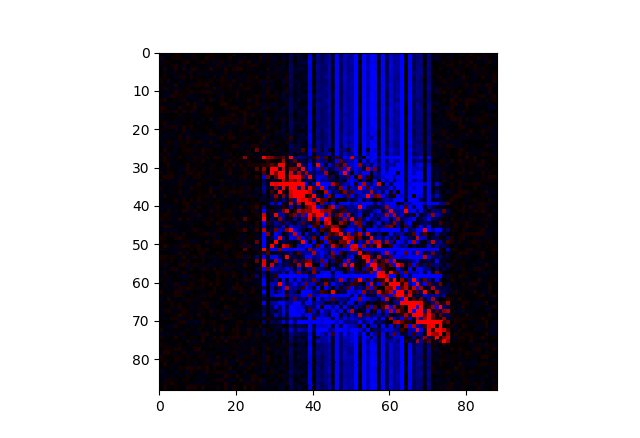
\includegraphics{figures/regression_weights.png}
    \caption{Here we plot the weights of the trained 1-step logistic regression model. Red indicates positivity and blue indicates negativity. As can be inferred, only notes 27 through 75 appear in the dataset. If a note is played in one time step, it is likely to be played in the next, and the probability of a note far away from the current note being played is low.}
\end{figure}

\begin{figure}
    \centering
    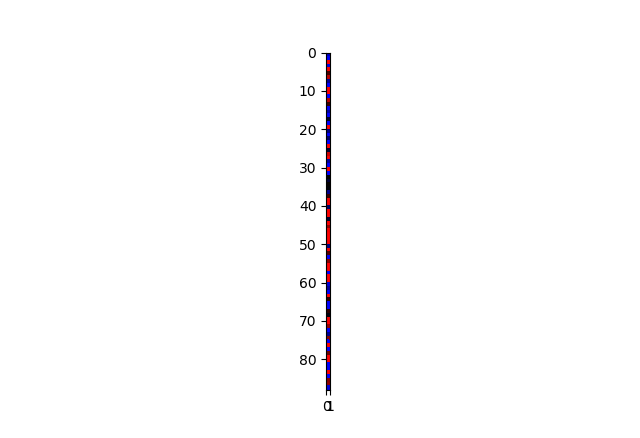
\includegraphics{figures/regression_bias.png}
    \caption{Here we plot the bias of the trained 1-step logistic regression model. The color scale is different from that of the weights.}
\end{figure}

Using the information encoded in the weights and bias, we should be able to recover the fact that all the songs were in C major, but I don't know how to do that yet.

\section{Latent LDS}

One can initialize a latent LDS so that it forgets everything at every time step and behaves like the regression model. Hopefully, this initialization is good for finding a superior solution to the problem using the LDS. We can also use the weights of the trained latent LDS to initialize a tanh RNN. First, we investigate the various ways the hidden weights of the latent LDS can be initialized.

\begin{figure}
    \centering
    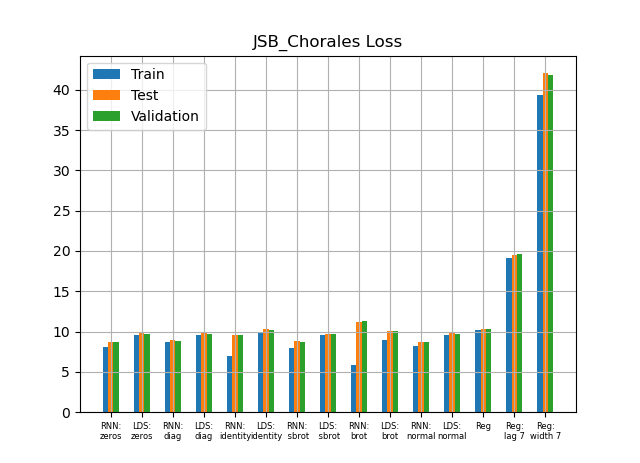
\includegraphics{figures/jsb_losses.png}
    \caption{Negative log likelihoods achieved by various models.}
\end{figure}

\begin{figure}
    \centering
    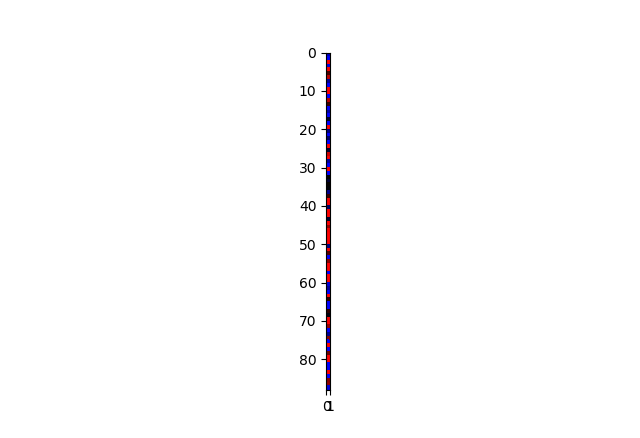
\includegraphics{figures/regression_bias.png}
    \caption{Accuracy achieved by various models.}
\end{figure}

\end{document}
